%%%%%%%%%%%%%%%%%%%%%%%%%%%%%%%%%%%%%%%%%%%%%%%%%%%%%%%%%%%%%%%%%%%%%%%%%%%%%%%%
%% MASTER'S THESIS                                                            %%
%%                                                                            %% 
%% Title (en): Multi-Agent Systems and Organizations                          %%
%% Title (cs): Multiagentní systémy a organizace                              %%
%%                                                                            %%
%% Author: Bc. Lukáš Kúdela                                                   %%
%% Supervisor: Prof. RNDr. Petr Štěpánek, DrSc.                               %%
%%                                                                            %%
%% Academic year: 2011/2012                                                   %%
%%%%%%%%%%%%%%%%%%%%%%%%%%%%%%%%%%%%%%%%%%%%%%%%%%%%%%%%%%%%%%%%%%%%%%%%%%%%%%%%

\section{PIM4Agents}

% PIM4Agents - authors
This section introduces the \textit{PIM4Agents} metamodel\footnote{For ``Platform-independent model for agents''.} \cite{Hahn07a}, \cite{Hahn07b} and \cite{Hahn08}, proposed in 2007 by Christian Hahn, Cristián Madrigal-Mora and Klaus Fischer from German Research Centre for Artificial Intelligence (Deutsches Forschungszentrum f\"{u}r K\"{u}nstliche Intelligenz, DFKI).
% Citation
We will present only a brief overview (distilled from \cite{Hahn07b}) since our work does not draw much inspiration from \textit{PIM4Agents}.

%% PIM4Agents %%%%%%%%%%%%%%%%%%%%%%%%%%%%%%%%%%%%%%%%%%%%%%%%%%%%%%%%%%%%%%%%%%

% PIM4Agents & MDA
\textit{PIM4Agents} has been specifically designed to be employed in the Model-driven engineering (MDE) software development methodology, more precisely in Model-driven architecture (MDA) by Object Management Group (OMG).
Apart from the platform-independent metamodel itself, the authors have proposed two platform-specific metamodels: \textit{JackMM} and \textit{JadeMM} for the \textit{JACK} and \textit{Jade} agent platforms respectively.
They have also described two sets of model transformations to convert PIMs to PSMs: \textit{PIM4Agents-to-JackMM} and \textit{PIM4Agents-to-JadeMM}.

%%%%%%%%%%%%%%%%%%%%%%%%%%%%%%%%%%%%%%%%%%%%%%%%%%%%%%%%%%%%%%%%%%%%%%%%%%%%%%%%
\subsection*{Core Model}

% Core metamodel
To support adaptability, \textit{PIM4Agents} is structured around a small core that can be augmented with extensions to model specific aspects of MASs, for example, security.
Figure~\ref{figure:pim4agents-metamodel} shows the core model.

% Agent
The metamodel, like previously introduced metamodels, is built around the concept of \textit{agent}, an autonomous entity capable of sensing its environment and acting upon it.
Each agent has access to a set of \textit{resources} from its surrounding \textit{environment} \cite{Hahn07b}.

% Behaviour
A \textit{behaviour} can be atomic or composed of sub-behaviours.
This way, a whole hierarchy of specific behaviours can be created.
A behaviour may also send or receive \textit{messages}\comments{FO} according to a \textit{protocol}\comments{FO}.
% Capability
A \textit{capability} allows to group conceptually related behaviours \cite{Hahn07b}.

% Role
A \textit{role} is an abstraction of the social behaviour of an agent in a given social context, usually a \textit{cooperation}\comments{FO}; it specifies the responsibilities of an agent in that social context.
% Cooperation
A \textit{cooperation} represents the interaction between agents playing the required set of roles.
% Protocol & Message
The detailed realisation of this interaction is described by a \textit{protocol} that specifies the \textit{messages} exchanged between the involved roles and at which point in time they are to be expected.
A protocol is executed by a set of behaviours sending and receiving messages in accordance to their roles.

% Organziation
Agents can take part in an \textit{organization}, a special kind of cooperation that also has the same characteristics as an agent.
Being a cooperation, an organization can have its own internal protocol that specifies how it coordinates its members.
Being also an agent, an organization can play roles in other organizations (\textit{super-organization}) and has capabilities which can be performed by its members, be they agents or other organizations (\textit{sub-organizations}).

% Figure: PIM4Agents metamodel
\begin{figure}[ht]
	\centering
	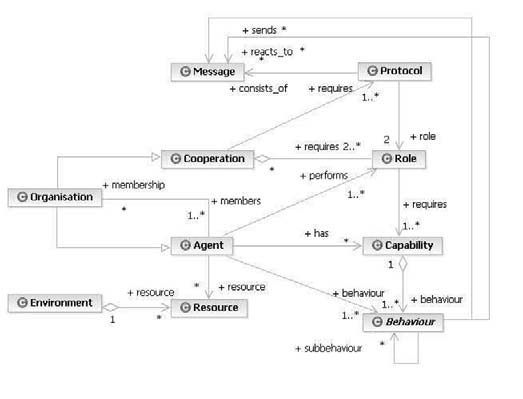
\includegraphics[width=0.6\textwidth]{images/pim4agents/pim4agents-metamodel.png}
	\caption{The \textit{PIM4Agents} core model \cite{Hahn07b}}
	\label{figure:pim4agents-metamodel}
\end{figure}

%%%%%%%%%%%%%%%%%%%%%%%%%%%%%%%%%%%%%%%%%%%%%%%%%%%%%%%%%%%%%%%%%%%%%%%%%%%%%%%%
\subsection{JadeOrgs}

\textit{JadeOrgs}, \cite{Madrigal-Mora08} and \cite{Madrigal-Mora09}, is an extension of the \textit{Jade} framework that implements the \textit{JadeMM} platform-specific metamodel.

\textit{JadeMM} is defined using Eclipse Modeling Framework (EMF) to exploit EMF's code generation facility.
Given a platform-independent model of a MAS (conforming to \textit{PIM4Agents}), the corresponding \textit{Jade/JadeOrgs} platform-specific model (conforming to \textit{JadeMM}) can be derived automatically.